%% Преамбула TeX-файла

% 1. Стиль и язык
\documentclass[utf8x, 12pt]{G7-32} % Стиль (по умолчанию будет 14pt)

% Остальные стандартные настройки убраны в preamble-std.tex
\sloppy

% 1. Настройки стиля ГОСТ 7-32
% Для начала определяем, хотим мы или нет, чтобы рисунки и таблицы нумеровались в пределах раздела, или нам нужна сквозная нумерация.
% А не забыл ли автор букву 't' ?
\EqInChapter % формулы будут нумероваться в пределах раздела
\TableInChapter % таблицы будут нумероваться в пределах раздела
\PicInChapter % рисунки будут нумероваться в пределах раздела

% 2. Добавляем гипертекстовое оглавление в PDF
\usepackage[
bookmarks=true, colorlinks=true, unicode=true,
urlcolor=black,linkcolor=black, anchorcolor=black,
citecolor=black, menucolor=black, filecolor=black,
]{hyperref}

% 3. Изменение начертания шрифта --- после чего выглядит таймсоподобно.
% apt-get install scalable-cyrfonts-tex

\IfFileExists{cyrtimes.sty}
    {
        \usepackage{cyrtimespatched}
    }
    {
        % А если Times нету, то будет CM...
    }


% 4. Прочие полезные пакеты.
\usepackage{underscore} % Ура! Теперь можно писать подчёркивание.
                        % И нельзя использовать подчёркивание в файлах.
                        % Выбирай, но осторожно.

\usepackage{graphicx}   % Пакет для включения рисунков

 % 5. Любимые команды
\newcommand{\Code}[1]{\textbf{#1}}

% 6. Поля
% С такими оно полями оно работает по-умолчанию:
% \RequirePackage[left=20mm,right=10mm,top=20mm,bottom=20mm,headsep=0pt]{geometry}
% Если вас тошнит от поля в 10мм --- увеличивайте до 20-ти, ну и про переплёт не забывайте:
\geometry{right=20mm}
\geometry{left=30mm}


% 7. Tikz
\usepackage{tikz}
\usetikzlibrary{arrows,positioning,shadows}

% 8 Листинги

\usepackage{listings}

% Значения по умолчанию
\lstset{
  basicstyle= \footnotesize,
  breakatwhitespace=true,% разрыв строк только на whitespacce
  breaklines=true,       % переносить длинные строки
%   captionpos=b,          % подписи снизу -- вроде не надо
  inputencoding=koi8-r,
  numbers=left,          % нумерация слева
  numberstyle=\footnotesize,
  showspaces=false,      % показывать пробелы подчеркиваниями -- идиотизм 70-х годов
  showstringspaces=false,
  showtabs=false,        % и табы тоже
  stepnumber=1,
  tabsize=4,              % кому нужны табы по 8 символов?
  frame=single
}

% Стиль для псевдокода: строчки обычно короткие, поэтому размер шрифта побольше
\lstdefinestyle{pseudocode}{
  basicstyle=\small,
  keywordstyle=\color{black}\bfseries\underbar,
  language=Pseudocode,
  numberstyle=\footnotesize,
  commentstyle=\footnotesize\it
}

% Стиль для обычного кода: маленький шрифт
\lstdefinestyle{realcode}{
  basicstyle=\scriptsize,
  numberstyle=\footnotesize
}

% Стиль для коротких кусков обычного кода: средний шрифт
\lstdefinestyle{simplecode}{
  basicstyle=\footnotesize,
  numberstyle=\footnotesize
}

% Стиль для BNF
\lstdefinestyle{grammar}{
  basicstyle=\footnotesize,
  numberstyle=\footnotesize,
  stringstyle=\bfseries\ttfamily,
  language=BNF
}

% Определим свой язык для написания псевдокодов на основе Python
\lstdefinelanguage[]{Pseudocode}[]{Python}{
  morekeywords={each,empty,wait,do},% ключевые слова добавлять сюда
  morecomment=[s]{\{}{\}},% комменты {а-ля Pascal} смотрятся нагляднее
  literate=% а сюда добавлять операторы, которые хотите отображать как мат. символы
    {->}{\ensuremath{$\rightarrow$}~}2%
    {<-}{\ensuremath{$\leftarrow$}~}2%
    {:=}{\ensuremath{$\leftarrow$}~}2%
    {<--}{\ensuremath{$\Longleftarrow$}~}2%
}[keywords,comments]

% Свой язык для задания грамматик в BNF
\lstdefinelanguage[]{BNF}[]{}{
  morekeywords={},
  morecomment=[s]{@}{@},
  morestring=[b]",%
  literate=%
    {->}{\ensuremath{$\rightarrow$}~}2%
    {*}{\ensuremath{$^*$}~}2%
    {+}{\ensuremath{$^+$}~}2%
    {|}{\ensuremath{$|$}~}2%
}[keywords,comments,strings]

% Подписи к листингам на русском языке.
\renewcommand*\thelstnumber{\oldstylenums{\the\value{lstnumber}}}
\renewcommand\lstlistingname{\cyr\CYRL\cyri\cyrs\cyrt\cyri\cyrn\cyrg}
\renewcommand\lstlistlistingname{\cyr\CYRL\cyri\cyrs\cyrt\cyri\cyrn\cyrg\cyri}

% Произвольная нумерация списков.
\usepackage{enumerate}


\begin{document}

\frontmatter % выключает нумерацию ВСЕГО; здесь начинаются ненумерованные главы: реферат, введение, глоссарий, сокращения и прочее

% Команды \breakingbeforechapters и \nonbreakingbeforechapters
% управляют разрывом страницы перед главами.
% По-умолчанию страница разрывается.

% \nobreakingbeforechapters
% \breakingbeforechapters

%% Также можно использовать \Referat, как в оригинале
\begin{abstract}

РПЗ: \total{page} стр., \total{myfigure} илл., 1 приложение.

\i{Ключевые слова:} распределенная система, детектирование спама.

\i{Объект разработки:} распределенная система обнаружения и фильтрации спама.

\i{Цель работы:} разработка распределенной системы обнаружения и фильтрации спама в протоколах POP3, IMAP, SMTP.

В качестве \i{технологической платформы} используется среда программирования PyCharm 2.0, язык Python.

\end{abstract}

%%% Local Variables: 
%%% mode: latex
%%% TeX-master: "rpz"
%%% End: 


\tableofcontents

\Defines % Необходимые определения. Вряд ли понадобться
\begin{description}
\item[Спам] Анонимные не запрошенные массовые рассылки электронной почты, то есть электронный эквивалент бумажной рекламной корреспонденции, засоряющей обычные почтовые ящики.
\item[SMTP] Сетевой протокол, предназначенный для передачи электронной почты в сетях TCP/IP.
\item[POP3] Сетевой протокол, используемый почтовым клиентом для получения сообщений электронной почты с сервера.
\item[MDA] Программа, принимающая входящие электронные письма и доставляющая их на электронный ящик получателя (если адрес назначения расположен на том же компьютере) или перенаправляющая их на другой почтовый сервер (если адрес назначения расположен на другом компьютере).
\item[MTA] Программа, которая передаёт сообщения от одного компьютера к другому по электронной почте.
\
\end{description}

%%% Local Variables:
%%% mode: latex
%%% TeX-master: "rpz"
%%% End:

\Abbreviations %% Список обозначений и сокращений в тексте
\begin{description}
\item{БД} --- база данных;
\item{ИП} --- интерфейс пользователя;
\item{МГТУ им. Баумана} --- Московский Госудраственный Технический Университет имени Н.Э. Баумана.
\item{ПО} --- программное обеспечение;
\item{РСОИ} --- распределенная система обработки информации;
\item{СУБД} --- система управления баз данных;
\item{ТЗ} --- техническое задание;
\item{IMAP} --- англ. Internet Message Access Protocol --- протокол прикладного уровня для доступа к электронной почте;
\item{MTA} --- англ. Mail Transfer Agent, Message Transfer Agent --- почтовый сервер;
\item{MDA} --- англ. Mail Deliver Agent --- агент доставки электронной почты;
\item{MUA} --- англ. Mail User Agent --- почтовый клиент;
\item{SMTP} --- англ. Simple Mail Transfer Protocol ---  простой протокол передачи почты;
\item{POP3} --- англ. Post Office Protocol Version 3 --- протокол почтового отделения, версия 3.

\end{description}

%%% Local Variables:
%%% mode: latex
%%% TeX-master: "rpz"
%%% End:


%\Introduction

Почтовая программа (клиент электронной почты, почтовый клиент, мейл-клиент, мейлер) — программное обеспечение, устанавливаемое на компьютере пользователя и предназначенное для получения, написания, отправки и хранения сообщений электронной почты одного или нескольких пользователей (в случае, например, нескольких учётных записей на одном компьютере) или нескольких учётных записей одного пользователя. Их предназначением является предоставление удобного пользовательского интерфейса для работы с электронной почтой. В рамках целой почтовой системы почтовые клиенты являются лишь интерфейсом пользователя. Когда пользователь отправляет письмо через почтовый клиент, это не означает, что данное приложение непосредственно 



Целью работы является создание всякой всячины. Для достижения поставленной цели необходимо решить следующие задачи:

\begin{itemize}
\item проанализировать существующую всячину;
\item спроектировать свою, новую всячину;
\item изготовить всякую всячину;
\item проверить её работоспособность.
\end{itemize}

Вот так-то. А этот абзац вставлен для визуальной оценки отступа от перечня до следующего абзаца.

\mainmatter % это включает нумерацию глав и секций в документе ниже

\chapter{Техническое задание}
\label{cha:analysis}
%
% % В начале раздела  можно напомнить его цель
%
Настоящее техническое задание разработано в рамках учебной программы по курсу <<Технология программирования>> на программное изделие <<Распределенная система обнаружения и фильтрации спама в протоколах POP3, IMAP, SMTP>>. Техническое задание выполняется в соответствии со стандартом ГОСТ 34.602-89 <<Техническое задание на создание автоматизированной системы>>.

\section{Наименование предприятия разработчика и заказчика системы}
Разработчиком системы является Сулимов Александр Сергеевич, студент группы ИУ7-104 кафедры ИУ-7 <<Программное обеспечение вычислительной техники и информационные технологии>> пятого курса очной формы обучения МГТУ им. Баумана.

Заказчиком системы является кафедра ИУ-7 <<Программное обеспечение вычислдительной техники и информационные технологии>> МГТУ им. Баумана (далее Заказчик).

\section{Основания для разработки}
Разработка ведется в рамках выполнения лабораторных работ по курсу <<Технология программирования>> и курсового проекта по курсу <<Распределенные системы обработки информации>> в соответствии с учебным планом МГТУ им. Баумана на 10-й семестр для факультета ИУ кафедры ИУ-7. При выполнении работы учитываются указания, описанные в методических пособиях \cite{metodRomanova}, \cite{metodKKrishenko}.

\section{Сроки выполнения работ по созданию системы}
В соответствии с требованиями Заказчика установлены следующие сроки (указываются номера недель, начиная с 6 февраля 2012 года):

\begin{enumerate}
	\item начало выполнения работ --- 3 неделя (20.02.2012 г.);
	\item конец выполнения работ --- 15 неделя (14.05.2012 г.).
\end{enumerate}

\section{Порядок оформления и предъявления результатов работы по созданию системы}
В \cite{metodKKrishenko} определены следующие требования к оформлению и защите проекта:

\begin{enumerate}
	\item в процессе разработки системы необходимо использовать выделенный Заказчиком репозиторий системы контроля версий;
	\item ответственное лицо со стороны Заказчика ведет контроль выполнения работы по репозиторию, учитывая количество коммитов, определяет процент выполнения проекта;
	\item результаты работ представляются в форме защиты проекта, на которой необходимо предъявить:
		\begin{enumerate}
			\item оформленную, прошитую и подписанную руководителем проекта пояснительную записку;
			\item презентацию в электронном виде в формате PDF;
			\item устаноленное и работающее программное обеспечение с исходными кодами, хранимыми в репозитории;
		\end{enumerate}
	\item при защите программное обеспечение должно быть установленно на компьютерах Заказчика;
	\item для защиты проекта создается комиссия из двух или более ответственных лиц со стороны Заказчика.
\end{enumerate}


\section{Актуальность разрабатываемой системы}
Представленные системы, позволяющие фильтровать почту он нежелательных сообщений, основываются на спам-фильтрах, которые имеют следующие недостатки:

\begin{enumerate}
\item{необходимо обучение;}
\item{история обучения локальная и относится к конкретному пользователю.}
\end{enumerate}

Настоящая разработка должна обеспечить передачу информации между пользователями о признаках обнаруженного спама. Распределенная система обнаружения спама позволит сократить время на обучение спам-фильтров для отдельных пользователей, тем самым повысит удобство использования почтовых клиентов.



\section{Краткое описание предметной области}
За последние десять лет сфера применения спама расширилась, а объем доставки - вырос значительно. Первое время спам рассылался напрямую на единичные адреса пользователей, и его было легко блокировать. Со временем появились высокоскоростные интернет-каналы, которые дали быструю и дешевую возможность массово рассылать спам-сообщения. Модемы пользователей не оснащались средствами защиты от несанкционированного доступа и могли использоваться злоумышленниками из любой точки планеты. Другими словами, модемы ничего не подозревающих пользователей рассылали огромные объемы спама.

Так продолжалось, пока производители аппаратного обеспечения не научились оснащать оборудование средствами защиты от спама, а спам-фильтры не стали более эффективными. Однако спам тоже эволюционировал: усовершенствовались не только способы рассылки, но и приемы, помогающие злоумышленникам обойти спам-фильтры. 

В ходе анализа предметной области были рассмотрены наиболее популярные спам-фильтры и другие механизмы, применяющиеся для фильтрации потока электронной почты от спама.


\section{Существующие аналоги}
В рамках настоящей работы был произведен анализ рынка программных продуктов, позволяющих фильтровать электронную почту от спама. Было выявлено, что существует множество решений позволяющих осуществлять определение нежелательной почты для конкретного пользователя. 

Существует два класса подобных продуктов:
\begin{enumerate}
	\item спам-фильтры на почтовых клиентах;
	\item спам-фильтры на почтовых серверах. 
\end{enumerate}

Спам-фильтры почтовых клиентов основаны на обработке входящих сообщений согласно заданным пользовательским правилам.  Почтовые сервера используют так называемые черные и серые списки доверенных адресов входящей почты.

Таким образом, распределенных систем, позволяющих осуществлять фильтрацию спама обнаружено не было.


\section{Назначение и цели создания системы}
Назначение разработки --- удовлетворить потребности клиентов (пользователей электронной почтой) в получении электронных писем, не относящихся к спаму.

Цели системы:
\begin{enumerate}
	\item информировать пользователя о том, что пришедшее сообщение относится к спаму;
	\item предоставлять пользователю возможность самостоятельно формировать спам-фильтры;
	\item обеспечить доставку писем, не относящихся к спаму.
\end{enumerate}

Таким образом, субъектами разрабытваемой РСОИ являются:

\begin{enumerate}
\item{система <<А>>}, почтовый клиент (MUA);
\item{система <<Б>>}, почтовый сервер (MTA);
\item{система <<C>>}, анти-спам сервер. 
\end{enumerate}

Перечисленные системы в дальнейшем будут также называться субъектами РСОИ или системами-участниками.

На рисунке ~\ref{fig:fig01} представлена структура предметной области и ее составные части.

\begin{figure}
  \centering
  \includegraphics[width=\textwidth]{inc/dia/rsoi-structure}
  \caption{Структура предметной области}
  \label{fig:fig01}
\end{figure}


\subsection{Система <<А>>}
Целью систем данного типа является предоставление удобного пользовательского интерфейса для работы с электронной почтой. С точки зрения почтовой системы представляют собой MUA --- программное обеспечение, устанавливаемое на компьютере пользователя и предназначенное для получения, написания, отправки и хранения сообщений электронной почты одного или нескольких пользователей (в случае, например, нескольких учётных записей на одном компьютере) или нескольких учётных записей одного пользователя. 

Системы <<А>> бывают двух типов в зависимости от протокола получения входящих сообщений:
\begin{enumerate}
\item{POP3;}
\item{IMAP.}
\end{enumerate}

Протокол POP3 подразумевает передачу входящих сообщений почтовым сервером и сохранение электронных писем на локальном компьютере пользователя. При использовании POP3 клиент подключается к серверу только на промежуток времени, необходимый для загрузки новых сообщений. При использовании IMAP соединение не разрывается, пока пользовательский интерфейс активен, а сообщения загружаются только по требованию клиента. Это позволяет уменьшить время отклика для пользователей, в чьих ящиках имеется много сообщений большого объёма.
Протокол POP требует, чтоб текущий клиент был единственным подключенным к ящику. IMAP позволяет одновременный доступ нескольких клиентов к ящику и предоставляет клиенту возможность отслеживать изменения, вносимые другими клиентами, подключенными одновременно с ним.


\subsection{Система <<Б>>}
Системы аккумулируют информацию необходимую для фильтрации электронной почты пользователя от спама. Целевые пользователи систем <<А>> должны зарегистрироваться в одной из систем типа <<Б>>. Такие системы получают информацию от пользователей относительно того, являются ли те или иные сообщения спамом или нет. В зависимости от полученных данных от пользователей в системах типа <<Б>> аккумулируется база данных, содержащая список адресов, с которых рассылаются спам-сообщения.

При получении почты системой <<А>> посылается запрос связанной с ней системой <<Б>>, которая должна классифицировать входящее сообщение на наличе спама.

Системы типа <<Б>> взаимодействуют между собой, таким образом пользователи, входящие в состав РСОИ, обладают суммарной информацией о всех спам-рассылках в рамках текущей сети. Так как с каждым пользователем системы <<А>>  в определенный момент времени связан лишь один антиспам сервер, то существует возможность составлять персональные спам-списки для каждого пользователя. 


\subsection{Система <<В>>}
 Системы данного типа отвечает за отправку почты и представляют собой почтовые сервера, которые обычно выполняют роль MTA и MDA. Некоторые почтовые сервера (программы) выполняют роль как MTA, так и MDA, некоторые подразумевают разделение на два независимых сервера: сервер-MTA и сервер-MDA (при этом, если для доступа к почтовому ящику используются различные протоколы — например, POP3 и IMAP, — то MDA в свою очередь может быть реализован либо как единое приложение, либо как набор приложений, каждое из которых отвечает за отдельный протокол).

 \section{Требования к системе}
 \subsection{Требование к системе вцелом}

 Разрабатываемое ПО должно удовлетворять следующим требованиям:

 \begin{enumerate}
 	\item все системы в РСОИ могут быть в одном или нескольких экземплярах, включение новой системы в РСОИ не должно приводить к нарушению работы других субъектов;
 	\item программное обеспечение для систем каждого типа должно 	поддерживать функционирование системы в режиме:
 		\begin{enumerate}
 			\item системы <<А>> --- периодическая работа в зависимости от желаний пользователя, в том числе поддерживать режим 24/7/365;
 			\item системы <<Б>> --- режим 24/7/365;
 			\item системы <<В>> --- режим 24/7/365.
 		\end{enumerate}
 	\item системы должны быть устойчивы к отключениям питания и другим техническим сбоям, которые могут привести к нарушению нормального фуннкционирования систем;
 	\item выход из строя одного субъекта РСОИ не должен приводить к сбою в работе других систем;
 	\item для корректного взаимодействия систем в РСОИ должен быть разработан протокол, однозначно определяющий содержание всех запросов и возможные сценарии совместной работы систем с указанием возможных состояний каждой из систем и состояний заявок в них.
 \end{enumerate}

 \subsection{Требования к функциональным характеристикам}
 К разрабатываему ПО выдвигаются следующие функциональные требования:
 \begin{enumerate}
 	\item время отклика на запрос пользователя не должно превышать 3 секунд;
 	\item время ожидания запросов для различных систем должно настраиваться с помощью конфигурационных файлов отдельно;
 	\item системы типа <<Б>> должны функционировать и поддерживать указанное время отклика для 50 одновременно подключенных клиентов-систем типа <<А>>;
 	\item указанные требования к временным задержкам должны соблюдаться для систем всех типов при одноверменной работе с 5-10 системами партнерами.
 \end{enumerate}

 \subsection{Требования по реализации}
 При разработке РСОИ участвующие системы реализуются в виде независимых программных продуктов, использующих общий протокол прикладного уровня для взаимодействия друг с другом. 

 К каждому из программных продуктов предъявляются следующие тербования:
 \begin{enumerate}
 	\item разрабатываемое ПО должно предоставлять удобный пользовательский интерфейс для работы администраторов и пользователей;
 	\item интерфейс систем должен быть реализован как WEB-интерфейс;
 	\item каждая заявка должна обладать уникальным идентификатором в рамках одного субъекта РСОИ;
 	\item в качестве транспортного протокола системы должны использовать почтовые протоколы SMTP для отправки POP3/IMAP для получения сообщений и протоколы удаленного вызова процедур XML-RPC;
 	\item в качестве языка разметки могут быть использованы языки XML, либо JSON;
 	\item для хранения данных о пользователях, сообщениях, спаме необходимо использовать СУБД Postgres. Непосредственный доступ к базе данных одной системы должен быть закрыт для систем партнеров и клиентов.
 \end{enumerate}


\section{Функциональные требования к системе}
\subsection{Функциональные требования к системам типа <<А>>}
Система <<А>> должна предоставлять следующие функции:
\begin{enumerate}
	\item аутентификация и авторизация пользователей;
	\item просмотр входящих сообщений пользователями;
	\item регистрация анти-спам сервера через панель настроек;
	\item оповещение связанного анти-спам сервера о наличии спам сообщений;
	\item просмотр сообщений, которые являются спамом по данным РСОИ;
	\item добавление адресатов в доверенный список, после чего сообщения от данных пользователей не классифицируются как спам;
	\item изменение способа получения входящих сообщений (протокол IMAP, POP3).
\end{enumerate}



\subsection{Функциональные требования к системам типа <<Б>>}
Система <<Б>> должна предоставлять следующие функции:
\begin{enumerate}
	\item аутентификация и авторизация пользователей;
	\item настройка спам-фильтров на стороне почтового сервера;
	\item настройка серых списков;
	\item настройка черных списков.
\end{enumerate}


\subsection{Функциональные требования к системам типа <<В>>}
Система <<В>> должна предоставить следующие функции:
\begin{enumerate}
	\item аутентификация и авторизация пользователей;
	\item просмотр списка подключенных почтовыхъ клиентов к данному анти-спам серверу;
	\item просмотр списка адресатов, признанных за спамеров;
	\item настройка списка адресатов;
	\item просмотр статуса вхощего сообщения;
	\item отмена обработки сообщения: доставка клиенту, удаление.
\end{enumerate}



\section{Входные параметры}
\subsection{Входные параметры систем типа <<А>>}
Система должна содержать следующую информацию о анти-спам сервере (система типа <<В>>):
\begin{enumerate}
	\item идентификатор системы;
	\item название системы;
	\item веб-адрес системы;
	\item адрес электронной почты системы;
	\item адрес XML-RPC сервера системы.
\end{enumerate}

Система должна содержать следующую информацию о почтовом сервере (система типа <<Б>>):
\begin{enumerate}
	\item идентификатор;
	\item название системы;
	\item веб-адрес системы;
	\item адрес электронной почты системы;
	\item адрес исходящей почты;
	\item адрес входящей почты и протокол ее получения.
\end{enumerate}

Система должна содержать следующую информацию о прокси-серверах POP3 и IMAP:
\begin{enumerate}
	\item веб-адрес сервера.
\end{enumerate}

Система должна содержать следующую информацию о пользователе:
\begin{enumerate}
	\item логин(уникальный идентификатор, адрес электронной почты);
	\item пароль;
	\item время последнего входа в систему;
	\item способ работы в настоящий момент времени (автономно, либо удаленно).
\end{enumerate}

Система должна содержать следующую информацию о входящем сообщении:
\begin{enumerate}
	\item уникальный идентификатор сообщения в рамках системы;
	\item наименование отправителя/получателя;
	\item контент сообщения (тема и тело сообщения);
	\item маркер спама, установленный пользователем (оценка от 0\% до 100\%);
	\item время получения сообщения.
\end{enumerate}

Система должна содержать следующую информацию об ошибках в работе:
\begin{enumerate}
	\item уникальный идентификатор ошибки в рамках системы;
	\item время возникновения;
	\item код ошибки;
	\item логин пользователя;
	\item адрес почтового сервера, адрес анти-спам сервера, адреса прокси серверов.
\end{enumerate}

\subsection{Входные параметры систем типа <<Б>>}

Система должна содержать следующую информацию о сообщении:
\begin{enumerate}
	\item уникальный идентификатор сообщения в рамках системы;
	\item адрес отправителя;
	\item адрес получателя;
	\item контент сообщения.
\end{enumerate}

Система должна знать следующую информацию об администраторах системы:
\begin{enumerate}
	\item логин;
	\item пароль.
\end{enumerate}

Система должна содержать следующую информацию об ошибках в работе:
\begin{enumerate}
	\item уникальный идентификатор ошибки в рамках системы;
	\item время возникновения;
	\item код ошибки.
\end{enumerate}

\subsection{Входные параметры систем типа <<В>>}
Система должна знать следующую информацию о сообщении:
\begin{enumerate}
	\item уникальный идентификатор сообщения в рамках системы;
	\item адрес отправителя;
	\item адрес получателя;
	\item контент сообщения.
\end{enumerate}

Система должна содержать следующую информацию об ошибках в работе:
\begin{enumerate}
	\item уникальный идентификатор ошибки в рамках системы;
	\item время возникновения;
	\item код ошибки;
	\item статус сообщений.
\end{enumerate}


\section{Требования к составу и параметрам технических средств}
Минимальные требования к программно-аппаратному обеспечению для рабочей станции системы типа <<А>>:

\begin{enumerate}
	\item тактовая частота  --- не менее $3,0 \text{ГГц}$; 
	\item оперативная память --- не менее $1 \text{Гб}$;
	\item требования к операционной системе:
	\begin{enumerate}
		\item Windows XP и старше;
		\item Mac OS X 10.5 и старше;
	\end{enumerate}
	\item свободное пространство на жестком диске не менее 10 Гб для операционной системы;
	\item свободное пространство на жестком диске не менее 200 Мб для программного обеспечения;
	\item Ethernet-адаптер стандарта 1000BASE-T для доступа к сети;
	\item веб-браузер;
	\item интерпретатор языка Python (для работы прокси).
\end{enumerate}

Минимальные требования к программно-аппаратному обеспечению для почтовых серверов систем типа <<Б>>:

\begin{enumerate}
	\item тактовая частота  --- не менее $2\times3,0$ ГГц; 
	\item оперативная память --- не менее $4$ Гб;
	\item требования к операционной системе:
	\begin{enumerate}
		\item Windows Server 2003 и старше;
		\item дистрибутив линукс с ядром версии 2.6:3.0;
	\end{enumerate}
	\item свободное пространство на жестком диске не менее 10 Гб для операционной системы;
	\item свободное пространство на жестком диске не менее 200 Мб для программного обеспечения;
	\item Ethernet-адаптер стандарта 1000BASE-T для доступа к сети;
	\item интерпретатор языка Python (для работы почтового сервиса);
	\item СУБД Postgres;	
	\item платформа Django для веб-интерфейса.
\end{enumerate}

Минимальные требования к программно-аппаратному обеспечению для анти-спам серверов систем типа <<В>>:

\begin{enumerate}
	\item тактовая частота  --- не менее $2\times3,0 \text{ГГц}$; 
	\item оперативная память --- не менее $4 \text{Гб}$;
	\item требования к операционной системе:
	\begin{enumerate}
		\item Windows Server 2003 и старше;
		\item дистрибутив линукс с ядром версии 2.6:3.0;
	\end{enumerate}
	\item свободное пространство на жестком диске не менее 10 Гб для операционной системы;
	\item свободное пространство на жестком диске не менее 200 Мб для программного обеспечения;
	\item Ethernet-адаптер стандарта 1000BASE-T для доступа к сети;
	\item интерпретатор языка Python (для работы прокси);
	\item платформа Django для веб-интерфейса;
	\item СУБД Postgres.
\end{enumerate}

\section{Сценарии функционирования системы}


\section{Состав и содержание работ по созданию системы}
В таблице \ref{tab:sostav} представлен состав работ по созданию РСОИ <<Распределенная система обнаружения и фильтрации спама в протоколах POP3, IMAP, SMTP>>. Перечень работ соответствует требованиям Заказчика.

\begin{table}[ht]
  \caption{Перечень работ по созданию РСОИ}
  \begin{tabular}{|p{0.70\textwidth}|c|}
  \hline
  Выполняемая работа & Срок выполнения\\
  \hline
  Исследование объектов автоматизации, сбор сведений о существующих аналогах & 1 неделя \\
  \hline
  Разработка технического задания & 4 неделя \\
  \hline
  Разработка пилотного проекта по выбранному варианту РСОИ & 6 неделя \\
  \hline
  Разработка окончательных решений по выбранным структурам, разработка конечных вариантов процедур и заглуушек систем-партнеров & 8 неделя \\
  \hline
  Разработка пользовательского интерфейса & 12 неделя \\ 
  \hline
   Создание документации & 12 неделя \\
  \hline
  Отладка проекта, подготовка к защите & 14 неделя \\
  \hline
  Защита проекта & 15 неделя\\
  \hline
  \end{tabular}
  \label{tab:sostav}
\end{table}


\section{Порядок контроля и приемки системы}
При разработке системы необходимо произвести следующие испытания:
\begin{enumerate}
	\item тестирование логики работы систем всех типов <<А>>, <<Б>>, <<В>>: при тестировании системы одного типа системы другого типа представляются в виде заглушек, работающих по строго заданным сценариям;
	\item тестирование нормальной совместной работы систем <<А>>, <<Б>>, <<В>>: проверяются различные сценарии работы при корректных входных данных, предполагаемые результаты работы сравниваются с реально полученными;
	\item испытание РСОИ на отказоустойчивость: имитирование таких событий как отключение питания, выход из строя других систем в составе РСОИ, поступление запросов с ошибочной или противоречивой информацией, поступление запросов в неверном формате и порядке.
\end{enumerate}


\section{Требования к документации}
Разработка, установка и внедрение системы должны сопровождаться следующими документами:

\begin{enumerate}
	\item руководство по установке, настройке систем всех типов при развертывании РСОИ;
	\item руководство по использованию систем <<А>> для пользователей;
	\item руководство по использованию систем <<Б>>, <<В>> для администраторов.
\end{enumerate}



%%% Local Variables:
%%% mode: latex
%%% TeX-master: "rpz"
%%% End:

%\chapter{Диаграммы}
\label{cha:design}

В данном разделе производится описание диаграмм, связанных с разработкой распределенной системы фильтрации спама.

\section{Диаграммы использования}

На рисунке~\ref{fig:usecase1} представлена диаграмма использования системы <<Почтовый Клиент>>.

\begin{figure}
  \centering
  [width=\textwidth]
  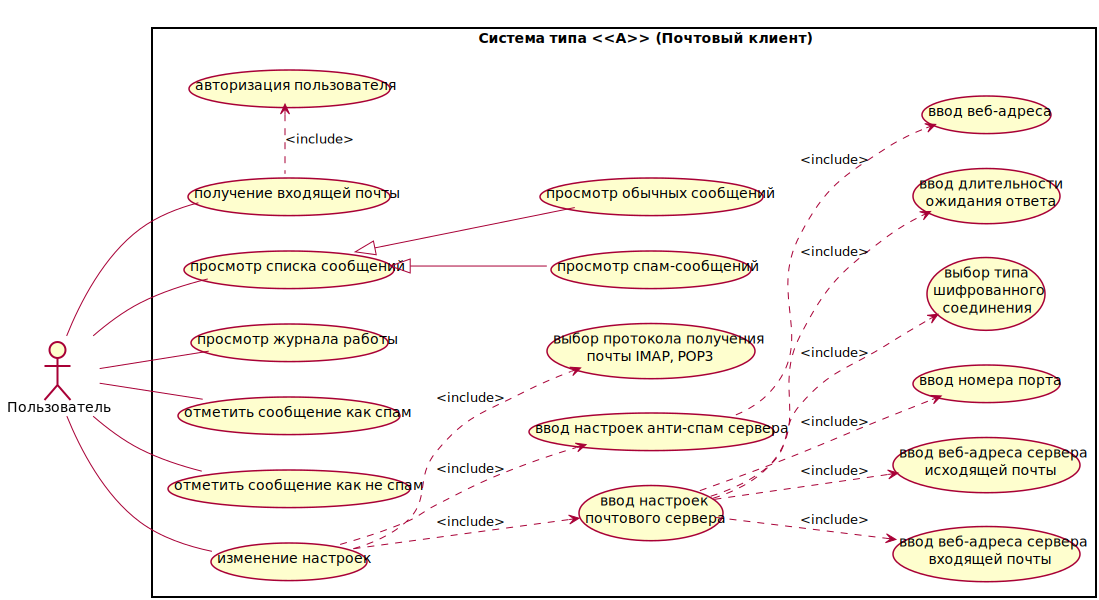
\includegraphics{inc/svg/use-case1}
  \caption{Диаграмма использования системы <<Почтовый Клиент>>}
  \label{fig:usecase1}
\end{figure}

На рисунке~\ref{fig:usecase2} представлена диаграмма использования системы <<Почтовый Сервер>>.

\begin{figure}
  \centering
  [width=\textwidth]
  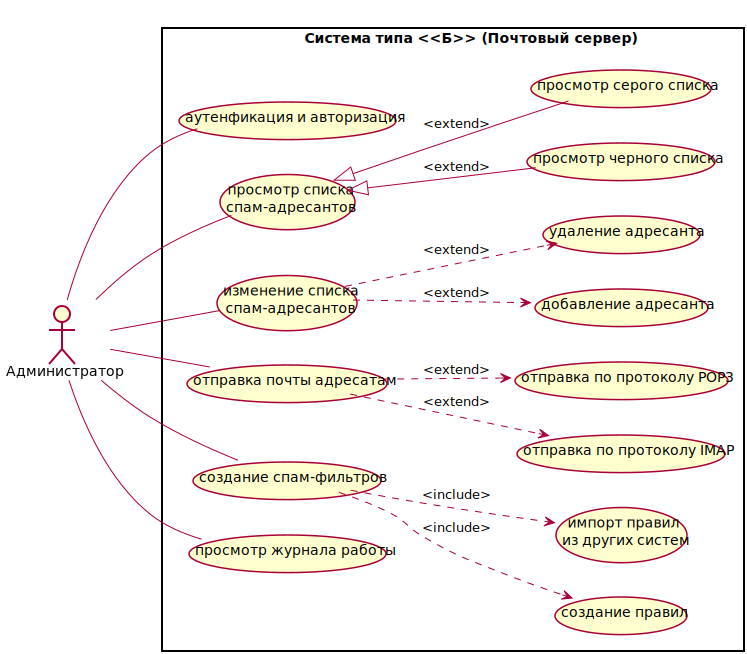
\includegraphics{inc/svg/use-case2}
  \caption{Диаграмма использования системы <<Почтовый Сервер>>}
  \label{fig:usecase2}
\end{figure}

На рисунке~\ref{fig:usecase3} представлена диаграмма использования системы <<Почтовый Сервер>>.

\begin{figure}
  \centering
  [width=\textwidth]
  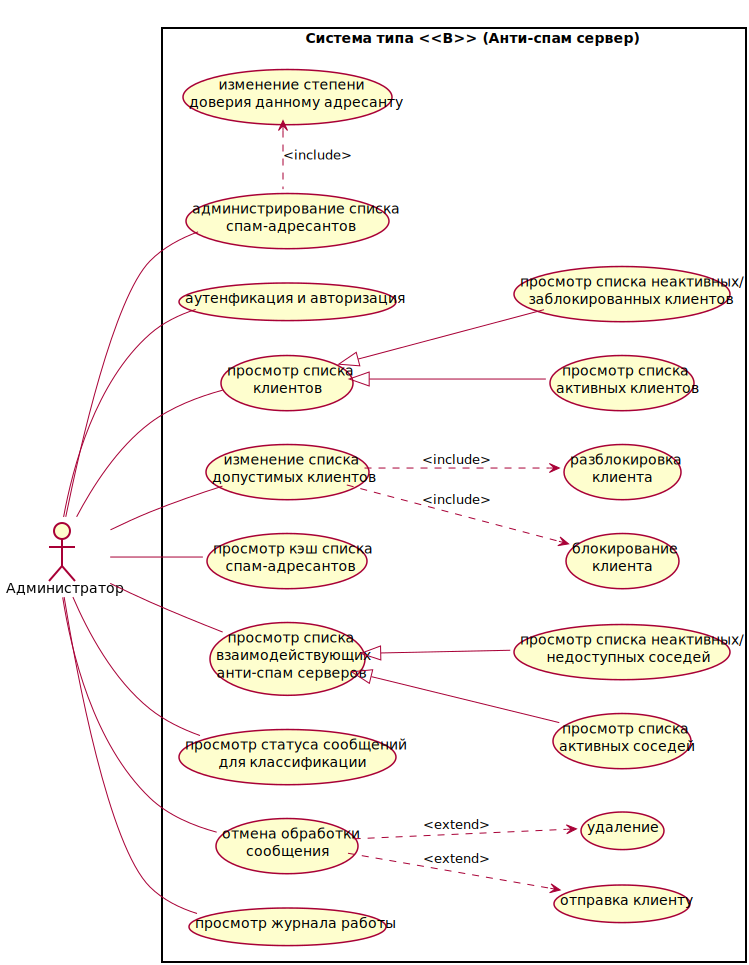
\includegraphics{inc/svg/use-case3}
  \caption{Диаграмма использования системы <<Анти-спам Сервер>>}
  \label{fig:usecase3}
\end{figure}

%\subsection{Блок-схема всякой ерунды}

%\subsubsection*{Кстати о заголовках}

%У нас есть и \Code{subsubsection}. Только лучше её не нумеровать.

%%% Local Variables:
%%% mode: latex
%%% TeX-master: "rpz"
%%% End:

%\chapter{Технологический раздел}
\label{cha:impl}

В данном разделе описано изготовление и требование всячины. Благодаря пакет \Code{underscore} эскейпить подчёркивание  не нужно (\Code{some_function}).

Для вставки кода есть пакет \Code{listings}. К сожалению, пакет \Code{listings} всё ещё
работает криво при появлении в листинге русских букв и кодировке исходников utf-8.
В данном примере он (увы) на лету конвертируется в koi-8 в ходе сборки pdf.

Есть альтернатива \Code{listingsutf8}, однако она работает лишь с
\texttt{\textbackslash lstinputlisting}, но не с окружением \Code{lstlisting}

Вот так можно вставлять псевдокод (питоноподобный язык определен в шаблоне):

\begin{lstlisting}[style=pseudocode,caption={Алгоритм оценки дипломных работ}]
def EvaluateDiplomas():
    for each student in Masters:
        student.Mark := 5
    for each student in Engineers:
        if Good(student):
            student.Mark := 5
        else:
            student.Mark := 4
\end{lstlisting}

Еще в шаблоне определен псевдоязык для BNF:

\begin{lstlisting}[style=grammar,basicstyle=\small,caption={Грамматика}]
  ifstmt -> "if" "(" expression ")" stmt |
            "if" "(" expression ")" stmt1 "else" stmt2
  number -> digit digit*
\end{lstlisting}

В листинге~\ref{lst:sample01} работают русские буквы. Сильная магия. Однако, работает
только во включаемых файлах, прямо в \TeX{} нельзя.

% Обратите внимание, что включается не ../src/..., а inc/src/...
% В Makefile есть соответствующее правило для inc/src/*,
% которое копирует исходные файлы из ../src и конвертирует из UTF-8 в KOI8-R.
% Кстати, поэтому использовать можно только русские буквы и ASCII,
% весь остальной UTF-8 вроде CJK и египетских иероглифов -- нельзя.

\lstinputlisting[language=C,caption=Пример (\Code{test.c}),label=lst:sample01]{inc/src/test.c}

% Для вставки реального кода лучше использовать \texttt{\textbackslash lstinputlisting} (который понимает
% UTF8) и стили \Code{realcode} либо \Code{simplecode} (в зависимости от размера куска).




Можно также использовать окружение \Code{verbatim}, если \Code{listings} чем-то не
устраивает. Только следует помнить, что табы в нём <<съедаются>>. Существует так же команда \Code{verbatiminput} для вставки файла.

\begin{verbatim}
a_b = a + b; // русский комментарий
if (a_b > 0)
    a_b = 0;
\end{verbatim}

%%% Local Variables:
%%% mode: latex
%%% TeX-master: "rpz"
%%% End:

%\chapter{Экспериментальный раздел}
\label{cha:research}

В данном разделе проводятся вычислительные эксперименты.
А на рис.~\ref{fig:spire01} показана схема мыслительного процесса автора...

\begin{figure}
  \centering
  \includegraphics[width=\textwidth]{inc/svg/pic01}
  \caption{Как страшно жить}
  \label{fig:spire01}
\end{figure}


%%% Local Variables:
%%% mode: latex
%%% TeX-master: "rpz"
%%% End:


\backmatter %% Здесь заканчивается нумерованная часть документа и начинаются ссылки и
            %% заключение

%\Conclusion % заключение к отчёту

В результате проделанной работы стало ясно, что ничего не ясно...

%%% Local Variables: 
%%% mode: latex
%%% TeX-master: "rpz"
%%% End: 


% % Список литературы при помощи BibTeX
% Юзать так:
%
% pdflatex rpz
% bibtex rpz
% pdflatex rpz

\bibliographystyle{gost780u}
\bibliography{rpz}

%%% Local Variables: 
%%% mode: latex
%%% TeX-master: "rpz"
%%% End: 


%\appendix   % Тут идут приложения

%\chapter{Картинки}
\label{cha:appendix1}

\begin{figure}
\centering
\caption{Картинка в приложении. Страшная и ужасная.}
\end{figure}

%%% Local Variables: 
%%% mode: latex
%%% TeX-master: "rpz"
%%% End: 

%\chapter{Еще картинки}
\label{cha:appendix2}

\begin{figure}
\centering
\caption{Еще одна картинка, ничем не лучше предыдущей. Но надо же как-то заполнить место.}
\end{figure}

%%% Local Variables: 
%%% mode: latex
%%% TeX-master: "rpz"
%%% End: 


\end{document}

%%% Local Variables:
%%% mode: latex
%%% TeX-master: t
%%% End:
